This chapter presents EgoLog, a mobile sensing framework for daily logging with audio and motion sensors. It instantiates the \textit{fusion} dimension of user--environment coupling: EgoLog combines activity cues from HMWs with environmental scenario context, using companion mobile devices when needed. The thesis emphasizes HMWs because they are suitable for day-long use and provide stable egocentric audio--motion observations. EgoLog selectively separates user-generated and environmental signals, then fuses them with scenario context to achieve robust recognition in the wild.
The following sections describe the motivation, system design, and evaluation of EgoLog.

\section{Introduction}
\label{sec:egolog_intro}
\begin{figure}[ht]
  \centering
    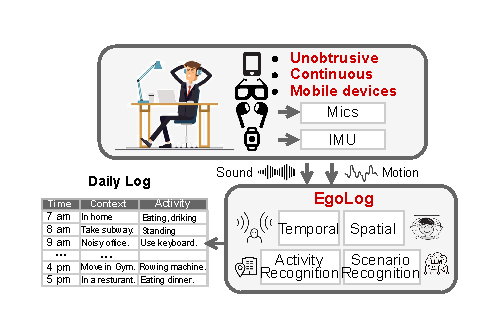
\includegraphics[width=1\linewidth]{chapters/egolog/figs/teaser.pdf}
    \caption{EgoLog uses microphones and an IMU on mobile and head-mounted devices for activity and scenario sensing.}
    \label{fig:egolog_teaser}
    \vspace{-1em}
\end{figure}

% HAR is important
Human activity recognition supports applications in physical and mental health monitoring, personalized healthcare, and daily routine analysis \citep{alam2014gesmart, gedam2021review}.
Smartphones and wearable devices can capture continuous sensor data during daily routines.
For example, motion data from an inertial measurement unit (IMU) can support human activity recognition because it reflects body movement. IMU-based systems have been developed for activities such as walking, standing, sitting, and lying~\citep{smartphonebased_recognition_of_human_activities_and_postural_transitions_341}.
Built-in microphones can also support acoustic scene recognition~\citep{martin2021low}, which provides contextual evidence for human activity.


% the limitation of previous work
However, existing HAR methods on mobile devices are limited to coarse-grained, scenario-constrained detection. For instance, step counting is a common application, but it fails to capture diverse activities such as cycling, swimming, or strength training. Although prior work has extended sensing to vital signs, gait analysis, and exercise recognition, these approaches often focus on isolated tasks rather than continuous daily monitoring.

% our problem/target
This chapter develops a mobile sensing system for ubiquitous devices, including earphones and smart glasses, to support continuous tracking of detailed egocentric human activities. The design models daily life from the user's perspective and moves beyond the recognition of short, isolated activities typically collected in laboratory settings. Fine-grained daily logging differs from conventional activity recognition in two ways:
\begin{enumerate}
    \item Daily life contains long-term activity structure, referred to here as ``scenarios.'' For instance, a user may spend an afternoon at the office while performing many related short-term activities.
    \item Daily life involves continuous interaction with the environment. Consequently, microphones capture sounds from the user, the environment, and other people. These environmental inputs can provide useful context, but they can also introduce noise.
\end{enumerate}


% device and modality
Several types of mobile devices are suitable for this task, including earphones, glasses, smartphones, and smartwatches. This thesis emphasizes head-mounted wearables because they are suitable for day-long use and provide stable egocentric observations, but the core audio--motion sensing design also applies to other mobile form factors. The available sensors can be roughly divided into two categories: visual and non-visual.
Visual sensors, such as cameras, can capture a first-person view rich with information. However, they are less practical for daily logging due to several limitations: 1) a limited field of view (FOV), 2) privacy concerns, and 3) high energy consumption for continuous sensing.
Instead, EgoLog uses non-visual sensors, namely motion and audio sensors. These sensors are widely available on smartphones, glasses, smartwatches, and earphones. As Fig. \ref{fig:egolog_teaser} shows, EgoLog continuously monitors a user's activities from an egocentric perspective and generates a daily log that includes both short-term activities and long-term scenarios.



% mobile devices have been a popular category of wearable devices that equip multiple sensors, such as microphones and IMUs. Being able to capture data from the user's ego view, mobile devices can be a desired platform for sensing detailed user-egocentric activities.
% First, earphone is the most popular wmobile devices with various applications including activity \citep{mollyn2022samosa}, speech \citep{he2023towards, dong2024rehearsse}, pose estimation \citep{duan2025argus}, eye tracking \citep{jiao2024medusa3d}, and vital signs \citep{chen2024exploring}.
% In 2025, there are more than 355 million mobile devices (e.g., earphones) sold, accounting for more than 60\% of wmobile devices worldwide \citep{Idc_2025}.
% Second, earphone is built with rich sensing capability, i.e., a microphone on each ear and an IMU. The sensors can capture stereo audio and motion that reflects egocentric information, such as user-induced speech and activities, and the location of environmental activities.
% Third, mobile devices are ideal for continuous sensing, the location of mobile devices is in the same place without the interference of the user's motion, and there is no blockage like a smartphone when it is placed in the pocket for most of the time.
% Besides, the average American young people use mobile devices more than 400 hours per year \citep{Ferjan_2022}, making it ideal for collecting continuous data.

This task introduces three challenges:
\begin{itemize}
    \item Existing mobile devices HAR models \citep{bhattacharya2022leveraging, gong2023mmg} lack the awareness of scenario information present in the real world. Specifically, user activities are driven by underlying reasons, and their distribution varies depending on the ``scenario.''  For instance, in an ``indoor cooking'' scenario, the ``jogging'' activity is less likely to happen.
    \item HAR models that depend on audio recordings are susceptible to interference due to the lack of spatial understanding. As a result, the audio data may lead to potential errors, which can be harmful for post-processing. For example, when detecting a ``clap'' activity based on sound, a nearby person's action could also trigger the model.
    \item Multi-modal fusion of audio and IMU is challenging and may not outperform a unimodal model \citep{huang2022modality}. Sensor heterogeneity weakens cross-modal alignment, as also observed in MMG-Ego4D \citep{gong2023mmg}. Effective fusion therefore requires models that identify when audio and motion are complementary.
\end{itemize}

To address these challenges, EgoLog uses the following design:
First, EgoLog recognizes long-term scenarios through temporal understanding, as detailed in Sec. \ref{sec:egolog_scenario}. This is achieved using a two-stage model: contrastive learning first projects audio and IMU features into a shared space to identify well-aligned segments as informative key frames; a sequence model then aggregates these key-frame features together with the original unimodal features for scenario recognition.

Second, EgoLog distinguishes user-generated activities from environmental sounds, including sounds produced by other people, through spatial understanding (Sec.~\ref{sec:egolog_localization}). The system formulates this as a sound localization task: near-field sounds are treated as user-centric events, while far-field sounds are treated as ambient background. A motion-aware localization model uses natural human movement and IMU readings to compensate for user motion and reduce spatial ambiguities such as near-far confusion.


Third, EgoLog introduces a multi-modal network for activity recognition that integrates audio, IMU, and scenario information (Sec.~\ref{sec:egolog_har}). Unlike short-term sensor data, the derived scenario captures longer-term behavioral patterns and provides high-level semantic cues for activity recognition.
The network uses dedicated unimodal backbones for feature extraction and a self-attention mechanism to dynamically fuse multimodal inputs, with scenario information encoded as a dense representation through a text encoder.

Finally, in Section \ref{sec:egolog_llm}, EgoLog introduces an edge-cloud framework assisted by a Large Language Model (LLM) for scenario recognition. The framework converts multi-modal data, including audio, IMU signals, sound localization outputs, and local scenario predictions, into contextual information for the LLM.
When the local model's prediction confidence is low, the edge device queries the cloud-based LLM. The refined scenario output is then used to update the local model over time.


We implemented and evaluated EgoLog on three large-scale public datasets, including Ego4D~\citep{grauman2022ego4d}, and a self-collected dataset covering multiple form factors, 10 participants, and 12 activities.
EgoLog improves activity recognition by 12\% and scenario recognition by 15\% over strong multi-modal baselines such as ImageBind~\citep{girdhar2023imagebind}, while keeping computation cost low.
The main contributions of this chapter are as follows:


\begin{itemize}
    \item
    EgoLog introduces an audio--IMU fusion method based on temporal and spatial understanding. It extracts scenario-level features through contrastive learning, aggregates them across short-term windows for scenario recognition, and integrates motion information with sound source localization for movement compensation.

    \item
    EgoLog develops an HAR method that takes both scenario context and raw sensor data as input. It uses scenario information to distinguish similar activities and uses sound-source estimates with audio--IMU correlation to separate user-generated sounds from background sounds.

    \item
    EgoLog introduces an LLM-assisted scenario recognition paradigm. Processed sensor data is fed into an LLM for high-level reasoning, and the LLM output is transferred back to the local device for on-device inference.

    \item
    EgoLog is evaluated on public datasets and a self-collected dataset, with an additional user study on the usefulness of generated daily summaries. The evaluation shows improvements of up to 15\% over the strongest baselines.
\end{itemize}

% \section{Related Work}

\label{sec:egolog_related}
\subsection{Motion Sensing for HAR}
IMU sensors in wearables and earables facilitate position tracking and user motion recognition, with their performance significantly impacted by sensor placement.
For example, LIMU-BERT \citep{xu2021limu} recognizes up to six activities with IMU recording of a smartphone.
Similarly, IMU on the wrist (e.g., smartwatch) can be used to recognize the basic activities \citep{chan2024capture}. 
Current motion sensing \citep{chan2024capture} only supports coarse-grained tasks, even with a large-scale dataset (>3000 hours), such as physical activity level (4 levels) or activities of daily life (10 activities).
Compared to smartphones and smartwatches, earables are a more reliable choice due to their relatively fixed position \citep{lyu2024earda, han2023headmon, han2023headsense, han2025headmon+}, as we illustrated before. Nonetheless, they share the same limitations in fine-grained motion sensing.

To enhance motion sensing, deploying multiple IMU sensors can enable precise full-body keypoint estimation with up to 17 IMUs. 
The pose of humans can be used to recognize fine-grained human activity, as demonstrated by MotionBERT ~\citep{zhu2023motionbert}. However, such an approach is impractical for everyday use. Instead, researchers propose leveraging commercial devices only, such as smartwatches, smartphones, and earables. For instance, combining multiple devices can enable fine-grained exercise activity recognition~\citep{stromback2020mm}. Similarly, IMUPoser achieves full-body pose estimation with just three IMUs~\citep{mollyn2023imuposer}. While using multiple devices improves performance, having all of them will have problems of high cost, user discomfort, setup complexity, and limited availability.

Another direction involves using pre-trained models to fuse IMU data with other modalities. Models like IMU2CLIP \citep{moon2023imu2clip} and ImageBind \citep{girdhar2023imagebind} link motion data to text or vision, enabling zero-shot recognition via retrieval. However, their performance on fine-grained tasks remains limited. Recently, Large Language Models (LLMs) have shown promise in reasoning over motion data \citep{ji2024hargpt, leng2024imugpt, xu2024autolife, ouyang2024llmsense}, often by converting sensor readings into text tokens for the LLM to process \citep{xu2024penetrative}.


% To further improve motion sensing, integrating advanced pretrained models that incorporate multiple modalities, such as text, offers a promising approach. Models like IMU2CLIP~\citepp{moon2023imu2clip} and ImageBind~\citep{girdhar2023imagebind} connect motion data to other modalities, enabling zero-shot activity recognition through retrieval. 
% However, their performance remains limited. For instance, IMU2CLIP \citepp{moon2023imu2clip} is restricted to four-class activity recognition, while ImageBind \citepp{girdhar2023imagebind} achieves only 25\% accuracy on fine-grained activity recognition.

% Recently, LLMs have demonstrated exceptional reasoning abilities when working on not only vision and text \citep{yang2024viassist, liu2023improved}, but also other modalities like motion \citep{ji2024hargpt, leng2024imugpt, xu2024autolife, ouyang2024llmsense}. For example, Penetrative AI \citep{xu2024penetrative} has shown that LLMs can also interpret sensor data such as accelerometers. 
% All of the above works convert the raw data into strings that can be easily accepted by LLM.

In summary, prior work on motion sensing either employs multiple IMU sensors or remains confined to coarse-grained activity recognition. Since IMU sensing inherently
lacks contextual or environmental information, which limits their ability to perform fine-grained HAR \citep{tong2020accelerometers}. Further advancements should focus on integrating additional modalities or external knowledge.

\subsection{Acoustic Sensing for HAR}
In addition to IMU sensors, acoustic sensors (microphones and speakers) are also commonly integrated into wearables and mobile devices. The use of a speaker allows acoustic sensing to be categorized into two approaches: active sensing (utilizing both the speaker and the microphone) and passive sensing (using only the microphone).

As the main research area of audio, there are multiple applications of passive audio sensing, including speech recognition and audio classification \citep{schmid2023efficient}. However, audio is related but does not directly reflect human activity. Instead, it relies on the sound caused by activity, which can be easily misled by a loudspeaker. As a result, audio-based HAR is often treated as a specialized form of audio classification \citep{cristina2024audio}.
In contrast, multi-channel passive sensing enhances spatial awareness by estimating the direction of arrival (DoA) of sounds using microphone arrays \citep{schmidt1986multiple, adavanne2018sound} or binaural earables \citep{yang2022deepear, krause2021joint}. While DoA provides useful context, it cannot confirm whether the source is human or differentiate the loudspeaker. To detect human presence, some approaches integrate feedforward microphones to capture vocal activity via head-related sounds \citep{zhang2024earsavas}, or use an IMU to capture the bone-conduction sound \citep{he2023towards}. However, they can only cover the vocal activity.

Different from passive sensing, active sensing analyzes transmitted acoustic waves and their reflections, enabling non-contact sensing.
For the context of human activity, we are more interested in 
sensing not only the facial movements \citep{dong2024rehearsse} with outward-facing speaker, such as upper body pose detection \citep{mahmud2023posesonic}, and gesture recognition \citep{yang2024maf}. However, the speakers are usually oriented inward or designed to be effective only in the near field to maintain user privacy, which hugely limits the performance in coarse-grained recognition. 

In summary, acoustic sensors in wearables enable rich information capture through either passive or active sensing. However, audio-based HAR is still limited, as passive sensing struggles to confirm human presence, and active sensing is constrained by practical considerations, necessitating multi-modal integration for improved performance.

\subsection{Multi-modal Sensing for HAR}
Multi-modal learning of audio and IMU data addresses limitations in motion sensing or acoustic sensing by leveraging the complementary strengths of both modalities. For instance, VibVoice \citep{he2023towards} uses bone-conduction vibration and audio in earables to distinguish a user’s voice from others. Similarly, \citep{min2018exploring} employs IMU for motion detection and a microphone for conversation detection, processed independently. Other wearables, such as wrist-mounted or head-mounted devices, also utilize multi-modal approaches; SAMoSA \citep{mollyn2022samosa, bhattacharya2022leveraging} integrates audio and IMU on smartwatches to recognize up to 26 activities. However, multi-modal learning is not universally superior, as its effectiveness depends on factors like data quality, modality correlation, and model design. 
For example, the fusion of audio and IMU on a diverse dataset like Ego4D \citep{grauman2022ego4d} can be challenging.
As demonstrated by MMG-Ego4D \citep{gong2023mmg}, where a multi-modal model for smart glasses underperformed compared to single-modal models in recognizing nearly 200 actions, highlighting that multi-modal approaches do not always guarantee improved performance \citep{huang2022modality}.

Beyond integrating audio and IMU sensors, incorporating additional knowledge sources can enhance motion sensing. For example, SAMoSA \citep{mollyn2022samosa} uses automatic context detection to trigger context-specific classifiers, though limited to predefined classes. Furthermore, the advanced LLMs facilitate multi-modal processing, either at the prompt level, incorporating IMU, GPS, Wi-Fi, or Bluetooth data \citep{yang2025contextagent, xu2024autolife,yang2024drhouse}, or at the token level, combining audio and IMU \citep{han2023onellm, girdhar2023imagebind}. While promising, those works lack explicit multi-modal fusion, especially for the heterogeneous multi-modal data from mobile devices.

In summary, the fusion of audio and IMU can be challenging since the correlation between them can be weak. While incorporating external knowledge or using powerful models like LLMs for fusion can enhance recognition, current methods still lack effective techniques for deeply integrating the heterogeneous data.
\section{Motivation Study}
\label{sec:egolog_measurement}
As discussed in Sec. \ref{sec:egolog_intro}, we mainly have three challenges towards a multi-modal HAR on mobile devices: 1) lack of scenario awareness, 2) being sensitive to ambient noise, and 3) fusion collapse. To explore these challenges and evaluate the potential for overcoming them, we conduct a series of experiments to analyze and demonstrate promising directions.

\begin{figure}
    \centering
    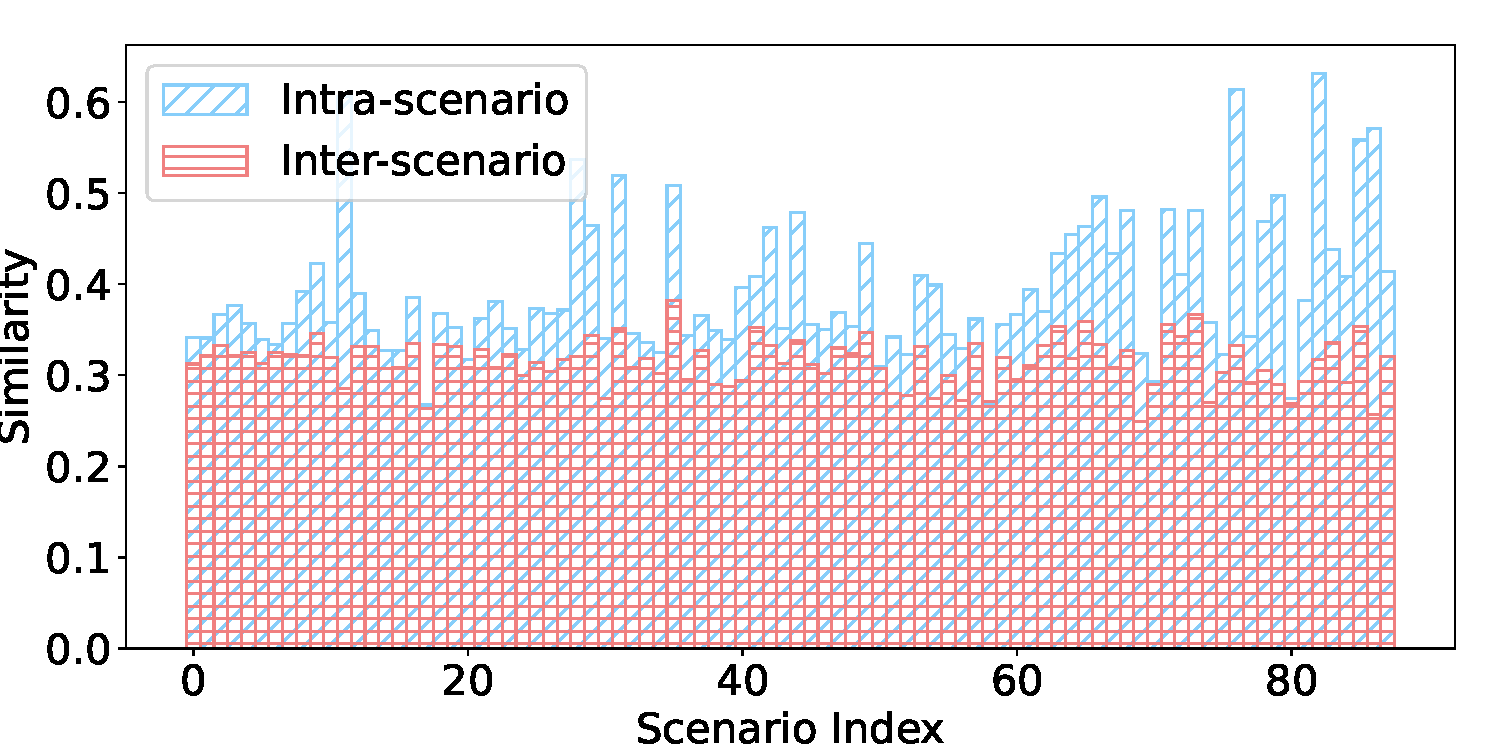
\includegraphics[width=0.8\linewidth]{chapters/egolog/figs/scenario_similarity.pdf}
    \vspace{-1em}
    \caption{Motivation for scenario understanding: 
    The similarity of embeddings for intra- and inter-scenario activities.}
    \label{fig:egolog_scenario_similarity}
    \vspace{-1em}
\end{figure}

\subsection{Scenario}
\label{subsec:scenario}
Scenario information refers to long-time activities (e.g., playing with a pet or working at home) that reflect the user's real-world behavior. Capturing such scenarios in datasets is challenging, as it requires volunteers to perform activities naturally, mimicking real-life conditions. Generally, scenario is the ensemble of multiple related and continuous activities with a realistic distribution, reflecting meaningful interactions with the environment.

To investigate the impact of scenario information on HAR, we use the Ego4D dataset~\citep{grauman2022ego4d}, which captures real-world activities through smart glasses equipped with IMU and audio sensors. The dataset provides annotations at both the window level (every 10 seconds) and the video level, represented as plain text. We treat window-level annotations as activity labels and video-level annotations as scenario labels that describe the broader setting of prolonged activities. To examine scenario properties, we use Sentence-BERT~\citep{reimers2019sentence} to generate text embeddings for activities across 91 scenarios. We then compute activity similarity both within scenarios (intra-scenario) and between scenarios (inter-scenario). Intra-scenario similarity measures the similarity of activities within the same scenario, while inter-scenario similarity compares an activity from one scenario to a randomly selected activity from a different scenario.

The results are shown in Fig.~\ref{fig:egolog_scenario_similarity}, revealing that the similarity within a scenario (intra-scenario similarity) is over 20\% higher than the similarity between different scenarios (inter-scenario similarity). This suggests that each scenario has a distinct distribution of activities. Specifically, a scenario effectively represents the user's daily log since it encompasses a longer time frame.
Additionally, we notice that the inter-scenario similarity is generally above 0.3, indicating that many basic activities (such as sitting and walking) are common across all scenarios. Therefore, it is crucial to eliminate the influence of these basic activities in scenario recognition, as they are present in every scenario.


In summary, the in-the-wild dataset shows that scenarios have distinct activity distributions, which can support scenario recognition through scenario-specific activities.


\subsection{Sound Location }
\label{subsec:embodied}
\begin{figure}
    \centering
    \begin{minipage}{0.48\linewidth}
        \centering
       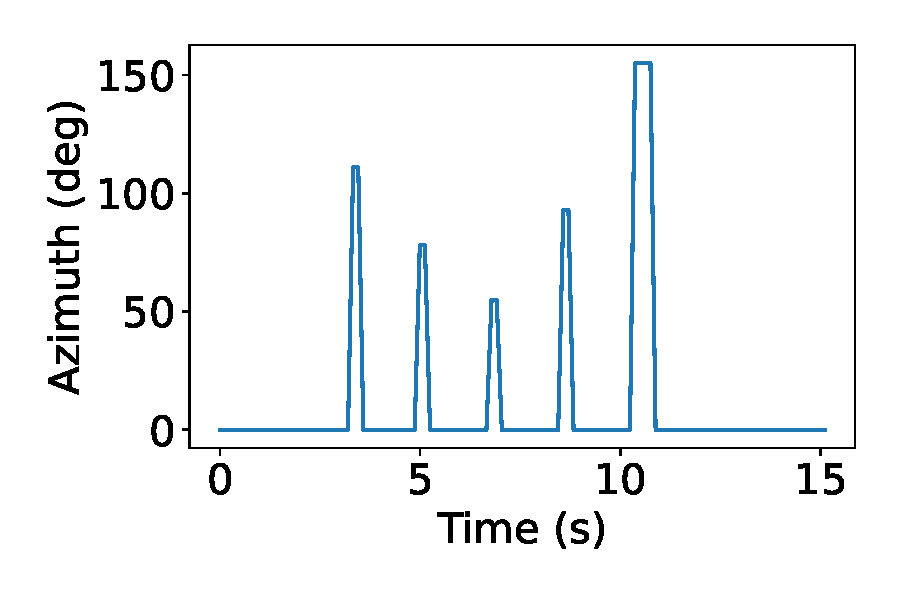
\includegraphics[width=\linewidth]{chapters/egolog/figs/baseline_result.pdf}
        \caption{Sound localization \citep{schmidt1986multiple} under motion}
        \label{fig:egolog_loc_move}
    \end{minipage}
    \hfill
    \begin{minipage}{0.48\linewidth}
        \centering
        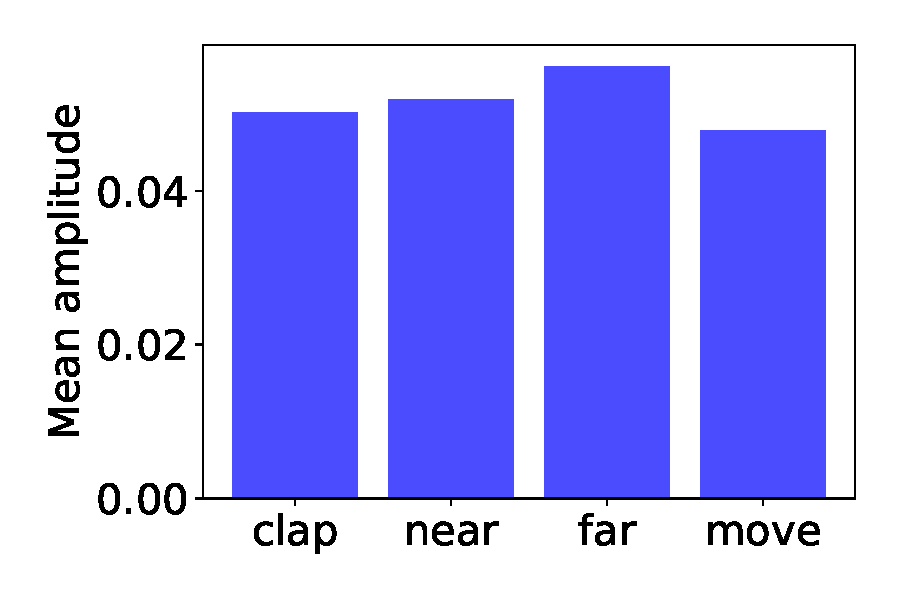
\includegraphics[width=\linewidth]{chapters/egolog/figs/amplitude.pdf}
        \caption{Sound volume may not related to distance.}
        \label{fig:egolog_amplitude}
    \end{minipage}    
    \vspace{-1em}
\end{figure}

\begin{figure}
    \centering
    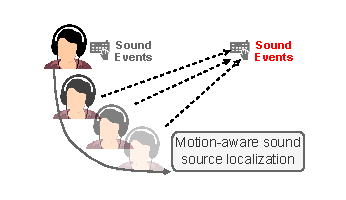
\includegraphics[width=0.75\linewidth]{chapters/egolog/figs/spatial_motivation.pdf}
    \vspace{-1em}
    \caption{Motivation for spatial understanding: estimate the distance of a sound event by motion.}
    \vspace{-1em}
    \label{fig:egolog_motivation_localization}
\end{figure}

In practice, recorded audio often includes far-field sound sources that are unrelated to the user’s activities, underscoring the importance of sound localization for effective HAR. Wearables that are consistently worn on the user’s head provide a stable and reliable position for capturing detailed ambient sound information. Additionally, modern wearables feature multi-channel recording capabilities, enhancing their spatial sensing potential.
In the following, we divide sound localization into direction and distance estimation, which we discuss as follows.

The estimation of sound direction is one of the mature, basic, but still challenging applications of a microphone array. The accuracy highly depends on the number of microphones, which is unfortunately not sufficient for most commercial devices. Considering the most common setting of stereo recording, there are mainly two problems: the deviation of direction (especially for front-back confusion) and estimation of sound distance, as illustrated in Fig. \ref{fig:egolog_motivation_localization}.
We envision that the above challenges may be solved by motion compensation. Specifically, we can aggregate the consecutive sound localization results along with the movement of the user (microphone) to refine the results or even get the distance.

To illustrate these challenges, we positioned a sound source in front of the user and used a binaural microphone with the algorithm from~\citep{schmidt1986multiple} to estimate direction of arrival, as shown in Fig.~\ref{fig:egolog_loc_move}. The user was instructed to move the body slightly and naturally. The estimate fluctuated around the true value of 90 degrees. To test whether sound volume is sufficient for differentiating near and far sources, we conducted an experiment with the sound source at different distances from the microphone. As shown in Fig.~\ref{fig:egolog_amplitude}, volume differences were not reliable across distances. The final bar in Fig.~\ref{fig:egolog_amplitude} also shows that user movement slightly affects amplitude. Multiple sound sources can further complicate volume-based distance estimation.

\subsection{Multi-modal Fusion }
\label{subsec:measure-fuse}

\begin{figure}
    \centering
     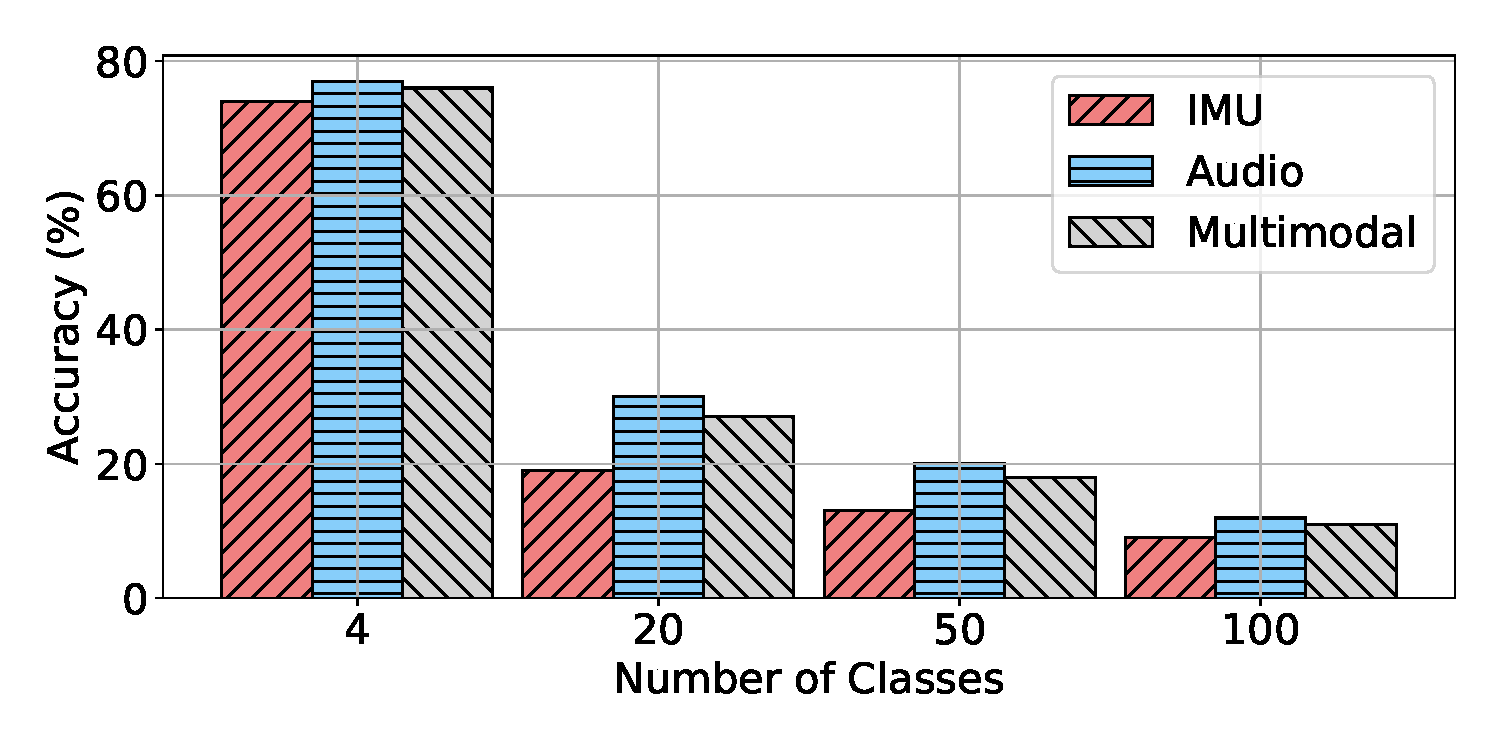
\includegraphics[width=.75\linewidth]{chapters/egolog/figs/num_class.pdf}
     \vspace{-1em}
      \caption{The performance of an existing activity recognition with different class numbers and modalities.}
    \label{fig:egolog_num_class}
    \vspace{-1em}
\end{figure}

To investigate scalability bottlenecks in activity recognition using wearables, we trained unimodal supervised models with audio and IMU data on the Ego4D episodic memory subset (200 activity classes). We used EfficientAT~\citep{schmid2023efficient} for audio and LIMU-BERT~\citep{xu2021limu} for IMU as feature extraction backbones, comparing them to a multi-modal model via late fusion. Activities were clustered into varying class numbers using Sentence BERT~\citep{reimers2019sentence} embeddings and K-Means~\citep{macqueen1967some}, following MMG-Ego4D~\citep{gong2023mmg}. Results (Fig.~\ref{fig:egolog_num_class}) show a significant performance drop as class numbers increase, indicating challenges in recognizing diverse activities with audio or IMU alone. Multimodal fusion often underperforms unimodal models, suggesting ineffective extraction of complementary features at larger scales.

\begin{figure}
    \centering
    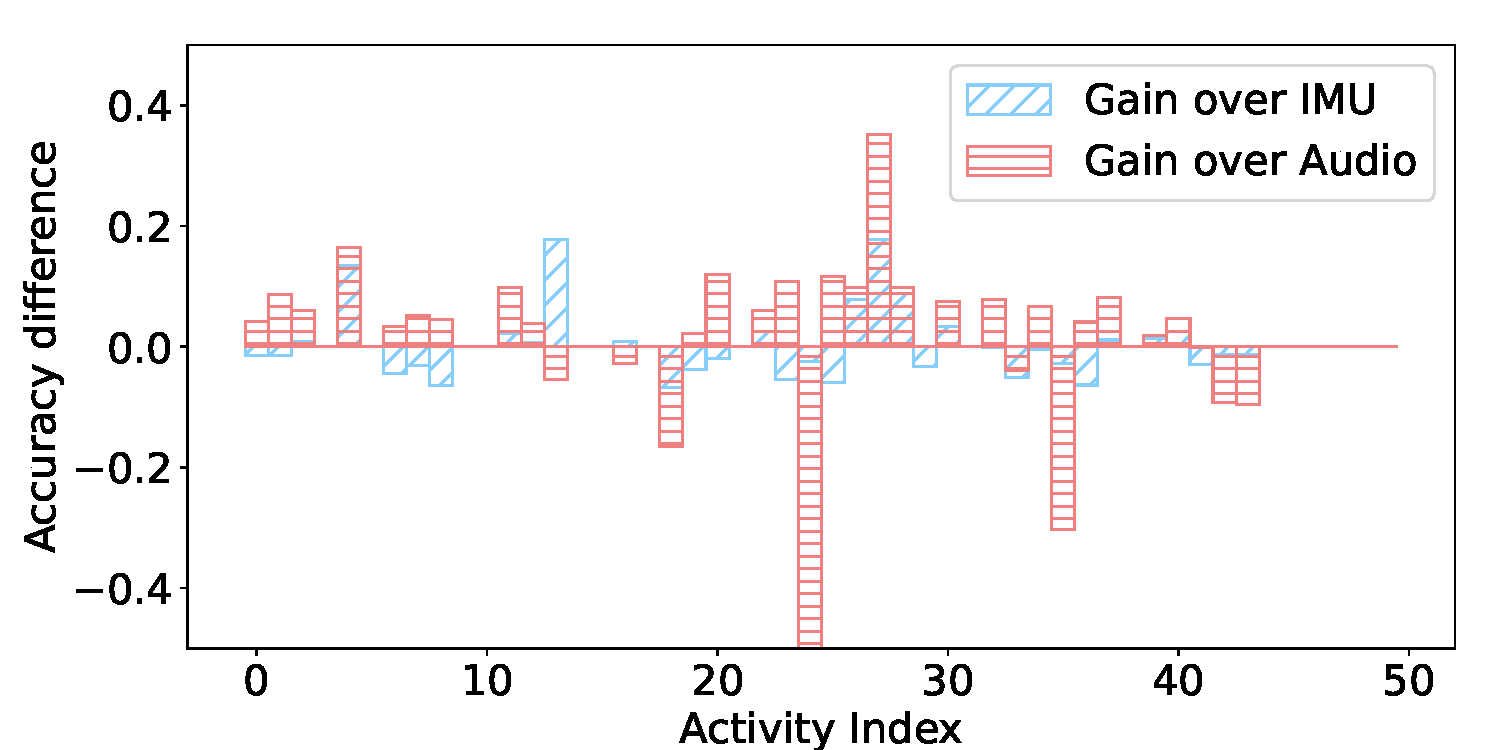
\includegraphics[width=.75\linewidth]{chapters/egolog/figs/activity_diff.pdf}
    \vspace{-1em}
    \caption{Performance gain from multi-modal fusion.}
    \label{fig:egolog_acc_gap}
    \vspace{-1em}
\end{figure}

Previous work~\citep{mollyn2022samosa} demonstrates that multi-modal learning can outperform the unimodal model due to the complementary nature of each other.
However, this finding does not apply to all cases. Another study~\citep{gong2023mmg} finds that multimodal learning with audio and IMU on Ego4D can perform worse than single-modality solutions. To investigate this result, we compared the accuracy of multimodal and unimodal models for each class, as shown in Fig.~\ref{fig:egolog_acc_gap}. The benefits of multimodal fusion fluctuate across both modalities, indicating that supervised multimodal learning cannot automatically select the appropriate modality for each activity.


To investigate whether LLMs can alleviate this problem, we evaluate ImageBind-LLM~\citep{han2023imagebind}, which converts both modalities into features and prepends them to text embeddings. We instruct the model with the prompt: ``<sensor> According to the audio and IMU reading on the earphone of the user, what is the activity of the user?'', where <sensor> denotes the inserted sensor features. Since LLM outputs can be random, we also constrain the prompt to one of the candidate activities. To reduce complexity, we select the top 30 activities from the Ego4D episodic memory subset. ImageBind-LLM achieves BERT-score precision, recall, and F1 score of 0.04, 0.07, and 0.05, respectively. Because this performance is low, we inspect the outputs and find that the LLM may not fully understand the multimodal fusion task.
We further test whether fine-tuning can address this problem by training an adapter~\citep{zhang2023llamaadapter} for ImageBind-LLM. The adapted LLM achieves BERT-score precision, recall, and F1 score of 0.47, 0.46, and 0.47, respectively. Although fine-tuning improves performance, the result remains below the level needed for practical use.

\section{System Design}
\begin{figure*}
    \centering
    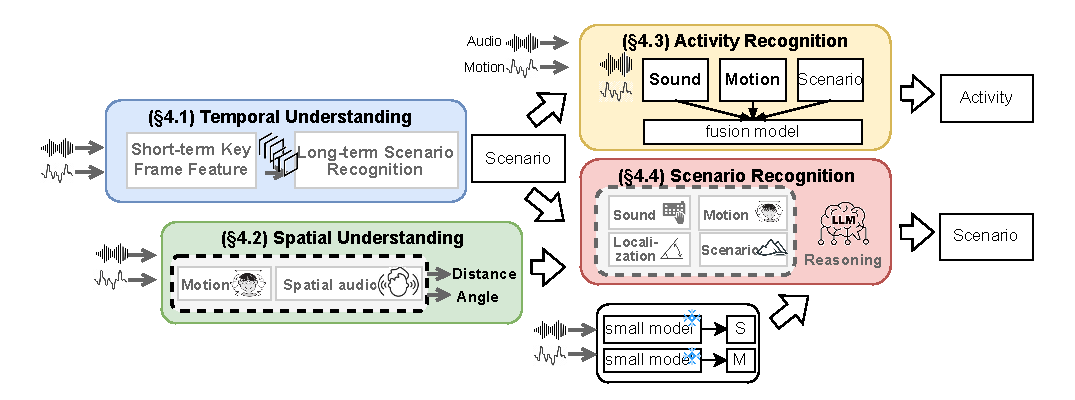
\includegraphics[width=0.8\linewidth]{chapters/egolog/figs/overview.pdf}
    \vspace{-1em}
      \caption{The system overview of EgoLog: the temporal and spatial understanding are two modules for multi-modal fusion, providing important input to the later modules to recognize activity and scenario}
      \vspace{-1em}
    \label{fig:egolog_system}
\end{figure*}

Figure~\ref{fig:egolog_system} provides an overview of EgoLog, a mobile system designed to capture egocentric daily logs over both long-term and short-term periods. 
Specifically, Section~\ref{sec:egolog_scenario} and Section~\ref{sec:egolog_localization} detail the fusion of audio and IMU data to achieve a deeper understanding of scenario (i.e., long-term descriptions) and spatial information (i.e., the relative location of sound sources). These insights serve as foundational clues for subsequent processing. 
In Section~\ref{sec:egolog_har}, we integrate the scenario information into the multi-modal activity recognition process, effectively mitigating modality collapse. Finally, Section~\ref{sec:egolog_llm} describes the use of an LLM as an expert to refine the scenario recognition from the previous stage; the resulting knowledge is subsequently transferred back to the local device.


\subsection{Temporal Understanding}
\label{sec:egolog_scenario}

\begin{figure}
  \centering
    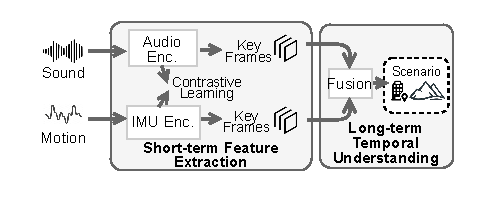
\includegraphics[width=1\linewidth]{chapters/egolog/figs/scenario.pdf}
    \vspace{-1em}
    \caption{Temporal understanding: we use contrastive learning to extract the cross-modal feature, which is important for the temporal-level fusion that recognize the scenario.}
    \vspace{-1em}
    \label{fig:egolog_scenario-recog}
\end{figure}

The measurement study indicates that recognizing many activities using IMU or audio data with an end-to-end model is difficult.
EgoLog therefore uses scenario recognition to provide prior information for activity recognition (Section~\ref{sec:egolog_har}). Scenario recognition also provides a useful high-level summary for daily logs.
As previously discussed, a scenario can be considered as a long-duration activity composed of multiple correlated sub-activities. To achieve accurate recognition, it is essential to develop an improved method for temporal analysis.
The pipeline is illustrated in Fig.~\ref{fig:egolog_scenario-recog}.


\subsubsection{Problem analysis}
Audio and IMU data have different properties and advantages. Their pretrained encoders are therefore optimized for different objectives. Simply merging their outputs may not produce the best results, as shown in Sec.~\ref{sec:egolog_measurement}; effective fusion must account for the heterogeneity of the two modalities.

We aim to tackle scenario recognition, which refers to identifying high-level human activities over an extended period (over 30 seconds). As detailed in Sec.~\ref{sec:egolog_measurement}, current pre-trained encoders already hold some scenario-level information, although they still fall short of ideal performance. A straightforward approach involves training a classification model using a dataset annotated with scenarios in an end-to-end fashion. Nonetheless, we have identified two persisting challenges: (1) the end-to-end model may struggle to generalize across different input lengths. (2) The performance might be inferior if scenarios are not included in the training data. Therefore, we propose training a new encoder for two modalities to obtain scenario-level features from brief time windows, which will then be applied in a secondary scenario recognition phase.

Given audio data and IMU data, the corresponding annotations for activity and scenario are assigned. Ideally, we could estimate activities individually and recognize scenarios accordingly. However, many activities may not relate to the audio or IMU data, such as silent motions that exceed the audio's capability.
Instead, we propose using two encoders: one for audio and one for IMU data. Their outputs would project the same feature space, representing features of the same scenario. Like activities, the two modalities may not always directly correlate with the scenario, so the mapping can fail sometimes. To address this, we can estimate the scenario by combining multiple windows of data, compensating for the sparsity of features.

\subsubsection{Contrastive learning}
Based on the preceding analysis, employing contrastive learning is optimal for capturing scenario-level features. Contrastive learning focuses on acquiring low-dimensional representations ($SE_i$) by differentiating between similar and dissimilar data samples. The method aims to group similar samples closely in the representation space while distancing dissimilar ones using the Euclidean distance. The efficacy of contrastive learning has been demonstrated in earlier research~\citep{han2023onellm, girdhar2023imagebind}. 
Within our framework, similarity and dissimilarity can be defined in two ways. Firstly, any data point aside from itself is deemed dissimilar. Secondly, data points within the same scenario are viewed as similar, whereas others are regarded as dissimilar. We expect that the first approach will yield more robust features, since it does not rely on explicit scenario annotations, and this will be assessed during the evaluation.

Regarding the network design, we employ two distinct deep neural networks to derive embeddings: LIMU-BERT~\citep{xu2021limu} for the IMU data and EfficientAT~\citep{lyu2024earda} for the audio input. Each sample spans a two-second window. The training of both encoders is based on the cross-entropy loss function, structured as follows:
\[
logits = (Audio_e \cdot IMU_e^T) \cdot \exp(\tau),
\]
where $Audio_e$ and $IMU_e$ refer to the features from two encoders, and $\tau$ refers to the learned temperature parameter \citep{chen2020simple}. Then, we get the loss using cross-entropy loss as follows:
\[
L = cross\_entropy\_loss(logits, label, axis=0).
\]

\subsubsection{Scenario recognition}
Assuming we extract the features from $Audio_e$ and $IMU_e$ by contrastive learning, they may not immediately convey the scenario as previously noted. We observe that a robust example in which both modalities relate to the scenario will exhibit a strong similarity between $Audio_e$ and $IMU_e$. This high similarity indicates that both modalities are effectively mapped into the same feature space, highlighting their importance as key features.
Conversely, low similarity suggests that the two modalities have not been successfully integrated into a unified representation of the scenario. Ideally, we would only keep frames with high similarity. However, the dynamics of execution can be problematic, introducing instability. Furthermore, it is difficult to set a definitive threshold to classify all frames below it as "useless."
Given the inherently weak correlation between audio and IMU, examples with high similarity may be rare. The model therefore needs to use as much information as possible from the available data.
To address this problem, we propose extending the key features along the temporal dimension. We integrate a sequence model—either an LSTM or a transformer—to compile features over time (as shown in the right section of Fig.~\ref{fig:egolog_scenario-recog}).
This two-stage architecture enables the model to capture both short-term and long-term dependencies within the features, thereby improving the accurate recognition of extended scenarios. Finally, a linear layer followed by a sigmoid activation function is used to predict the probability for each scenario.

\begin{figure}
  \centering
    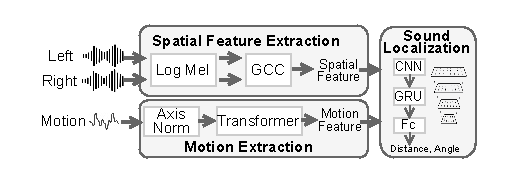
\includegraphics[width=1\linewidth]{chapters/egolog/figs/localization.pdf}
    \vspace{-1em}
    \caption{Spatial understanding: we differentiate sound by location by the combination of spatial audio and motion, leveraging the natural but random movement of the user.}
    \label{fig:egolog_seldnet}
    \vspace{-1em}
\end{figure}


\subsection{Spatial Understanding}
\label{sec:egolog_localization}
Existing activity recognition methods by audio are often misled by environmental events.
As illustrated in Sec. \ref{sec:egolog_measurement}, it is not enough to use sound volume to differentiate the near-field and far-field sound. Here, we are interested in the near-field sound because of the close correlation between it and the user's interaction with the environment. 

\subsubsection{Sound localization}
The location of sound can be estimated by a multi-channel microphone array. 
Specifically, the time of arrival of the sound source for one microphone is: \(t_i = \frac{\sqrt{(x_s - x_i)^2 + (y_s - y_i)^2}}{c}\), where the location of microphones $\mathbf{p}_i = (x_i, y_i)$, $i = 1, \ldots, N$, and a sound source at $\mathbf{s} = (x_s, y_s)$.
Since the start time of the sound source is unknown, the system can only obtain the time difference of arrival (TDoA) between two microphones, such as $i$ and $j$. With only two microphones on binaural earables, this yields a single equation, which is insufficient to resolve front--back confusion reliably.

Building on the work of SELDNet \citep{adavanne2018sound} and DeepEar \citep{yang2022deepear}, we propose a neural network-based binaural localization. Overall, our model performs an 8-class classification, distinguishing between four directions (front, left, right, back) and two distance categories (near and far). The binaural audio input, is converted to two log-Mel spectrograms and generalized cross-correlation coefficients of spectrograms, combined along the channel dimension to form spatial features with shape \( B \times 3 \times T \times 64 \), where \( B \) is the batch size and \( T \) is the number of frames. We process the audio feature with three convolutional layers, transforming it to (B, 128, T/5, 64). Then it is followed by a GRU layer, multi-head attention (resulting in B, 128, T/5, 64), and a linear layer that outputs (B, T/5, C).


\subsubsection{Movement compensation}

As illustrated in the motivation study, user movement can improve spatial understanding. Similar ideas have been used in prior work~\citep{zhu2021localizing, seo2022ross}, but these approaches require either explicit user gestures or a fully controllable robot. EgoLog instead uses natural, unintentional body movements that occur in daily life.

To realize this, we introduce an end-to-end method where IMU data—structured as (B, 6, T) and comprising both accelerometer and gyroscope measurements—is processed through two transformer layers. This module outputs a representation of shape (B, 384, T), which is then passed through a linear layer to produce an output of size (B, T/5, C). The resulting features are subsequently concatenated with the output from the GRU module.
The overall model performs an 8-class classification (C=8), distinguishing between four spatial directions (front, left, right, back) and two distance categories (near and far).

EgoLog cannot assume that only one sound source exists. Multiple sound sources may overlap, and both sound localization and audio recognition can be multi-label. This creates an association problem, which is addressed in a later section.

\subsection{Scenario-aware Activity Recognition}
\label{sec:egolog_har}

\begin{figure}
    \centering
    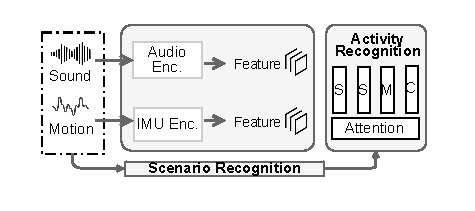
\includegraphics[width=1\linewidth]{chapters/egolog/figs/activity_recognition.pdf}
    \vspace{-1em}
    \caption{Multi-modal activity recognition: We extract features from each individual modality (uni-modal features), combine them with the scenario information derived from temporal understanding, and merge them at the token level for final activity recognition.}
    \vspace{-1em}
    \label{fig:egolog_activity_recognition}
\end{figure}

The methods outlined in Sec. \ref{sec:egolog_scenario} and \ref{sec:egolog_localization} offer a promising path for audio-IMU fusion. Next, we propose to integrate them into HAR.

Our proposed multi-modal network consists of two main components: unimodal backbones and a fusion module. The unimodal backbones include separate feature extractors that gather features from each input modality. The fusion module is designed to combine and aggregate these features from the unimodal backbones, resulting in a fused output that denotes the activity of the user. Although the design described above shows promise, it shares similar input and output characteristics with those presented in Section \ref{sec:egolog_measurement}, which has already been validated. As a result, it may not perform well in human activity recognition due to a lack of multi-modal correlation.

There are two common approaches for fusing modalities: using a multi-layer perceptron to process concatenated representations, or using a Transformer-based fusion module that processes a sequence of tokens from different modalities~\citep{gabeur2020multi}. EgoLog uses the Transformer-based design because attention can scale to a variable number of input tokens.
This flexibility is particularly important, as our multi-modal model needs to handle data with a varying number of modalities (more than only audio and IMU) for the task. Specifically, suppose the scenario information is a feature with the same dimension as other modalities, the transformer module can easily integrate it.
The final output of the fusion module is calculated by averaging the output tokens, rather than relying on the CLS token. The formulation of the token for one modality $Z_m$ is below:
\[
Z_m = (Encoder_m(S_m), e_m), \quad Z=f(Z_1, Z2, Z_3...)
\], where \( m \) represents each modality, which includes audio, IMU, and text. The term \( e_m \) denotes the learnable embedding specific to each modality. The transformer fusion module will combine multiple \( Z_m \) tokens and produce a unified \( Z \) feature with consistent dimensions. 
Similar to the previous section, we keep the audio and IMU encoder used for scenario recognition since both of them are lightweight and can be deployed on a mobile device.
By default, we use the standard transformer with a number of layers of 2. 

Next, we extend the multi-modal model that can handle not only the audio and IMU, but also other auxiliary information, such as scenario:
\begin{itemize}
    \item Specifically, we collect scenario information from Sec. \ref{sec:egolog_scenario} in textual form. To integrate it, we use the ImageBind \citep{girdhar2023imagebind} text encoder to map this information into the same feature space as the other modalities. Note that the text embeddings can be precomputed and stored to reduce computational overhead for each scenario. When multiple scenarios are detected, we concatenate their corresponding text representations.

    \item For spatial information from Sec. \ref{sec:egolog_localization}, we treat it as an indicator for interference detection. When far-field sound is detected with a confidence score exceeding 0.9, the audio recording is considered unreliable. In such cases, we can either discard the audio recording and rely solely on motion sensing or apply distance-based sound extraction \citep{chen2024hearable} to retain only the near-field sound.
\end{itemize} 


\subsection{LLM-assisted Scenario Recognition}
\label{sec:egolog_llm}
\begin{figure}
    \centering
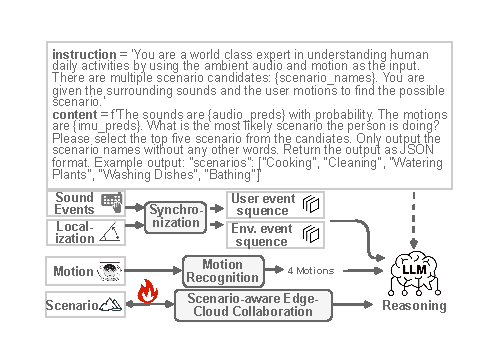
\includegraphics[width=1\linewidth]{chapters/egolog/figs/llm_reasoning.pdf}
\vspace{-2em}
    \caption{LLM-assisted scenario recognition: Utilizing prior outputs, we differentiate sound events into those originating from the user and those from the environment. We then combine it with motion and scenario recognition results and feed it into an LLM for reasoning (the upstream process). The LLM's output is then used as a pseudo-label to re-train the local model (the downstream process).}
    \vspace{-1em}
    \label{fig:egolog_llm_reasoning}
\end{figure}


As discussed in Section~\ref{sec:egolog_measurement}, LLMs may be suboptimal for direct activity recognition. They are better suited to higher-level scenario recognition, where longer data sequences provide richer context. This is consistent with Section~\ref{sec:egolog_scenario}, where longer sequences also benefit multimodal fusion. As illustrated in Fig.~\ref{fig:egolog_llm_reasoning}, EgoLog formats five-second sensor windows as text and uses tailored prompts to guide LLM-based scenario recognition. The LLM output can then refine local scenario predictions. All LLM processing is performed in the cloud so that the local EgoLog model remains lightweight.
 
\subsubsection{Prompt design}
Existing studies primarily use LLM reasoning on text-like data. This subsection introduces how EgoLog converts multimodal audio and motion signals into prompts for LLM-based scenario reasoning, as illustrated in Fig.~\ref{fig:egolog_llm_reasoning}. Instead of retraining the LLM or adding an adapter, EgoLog uses a specialized prompt with demonstrations that describe how to reason over sensor-derived context.
The prompt is structured as follows: “You are an expert in human activity analysis. You will receive audio and IMU recognition results, including extra information on potential scenarios. Using this information, reason and refine the person’s scenario. The scenario must be one of the following categories: [List of categories]. Your output must be a single line containing just one word or phrase.”
This prompt, along with the formatted input data as shown below, is fed to the LLM.

\paragraph{Audio.} 
We employ a pre-trained audio recognizer \citep{schmid2023efficient} to transcribe audio into text by selecting the top three predictions. The output is structured as "the detected audio classes are <class1, prob1>, <class2, prob2>, <class3, prob3>...", where each entry is referred to as a sound event. To minimize noise, we retain only the top five predictions with a confidence score exceeding 0.3.
Since the classifier's label set is based on the AudioSet ontology, the defined classes are highly fine-grained, often resulting in multiple similar classes with comparable probabilities. This lack of discriminative power hinders effective reasoning. To address this, we apply a two-level hierarchical clustering of the classes to their parent categories, reducing the total number of classes from 416 to 50 and improving generalization.

\paragraph{IMU.} 
Following the IMUCLIP approach \citep{moon2023imu2clip}, we classify IMU data into four activities: walking, moving, standing up, and sitting down. While previous works have demonstrated the ability to recognize more fine-grained activities using IMU data, their generalization capabilities remain questionable due to reliance on scenario-constrained datasets.

\paragraph{Spatial.}
EgoLog uses spatial information from Sec.~\ref{sec:egolog_localization} by applying different processing strategies to near-field and far-field audio inputs. For near-field sounds, the prompt states that the sound event occurs near the front of the user and is likely related to human activity. For far-field sounds, the prompt states that the sound event occurs at the estimated sound location.
When both near-field and far-field sounds are detected, it is unclear which event is near or far. As a result, we can turn on the distance-based sound separation \citep{chen2024hearable} that separate the audio into two and perform the sound recognition, respectively. We leave the optimization of the separation in the future work since it is unrelated to the main body of EgoLog.




\subsubsection{Scenario-aware LLM Assistance}

We define an upstream and downstream collaboration paradigm where the edge device seeks assistance from a cloud-based LLM, rather than naively querying the response.

For the upstream path, EgoLog uses the scenario recognition capability of LLMs, especially for out-of-domain data. The scenario estimated by the edge device is treated as a noisy reference that provides preliminary information to the LLM. The prompt includes this estimate and its confidence score.
Specifically, the estimated scenarios are added to the prompt, augmented by the text: "the preliminary scenario estimation is <scenario, confidence>."
However, frequent queries to the cloud service raise concerns about cost, privacy, and latency. Ideally, all modules of EgoLog should be executable on a mobile device if the performance is sufficient. Consequently, we propose a collaborative framework that strategically uses the cloud LLM to enhance the local model. Specifically, a confidence threshold (0.5) is set for the local scenario recognition model. A cloud query is triggered only when the local model's confidence is low.

Complementing the upstream process, we also propose a downstream collaboration where the cloud LLM's output can assist the local model. EgoLog sends the derived textual representation of an uncertain case, rather than its raw audio or IMU samples, to the LLM. The corresponding local sample and the LLM's refined label are then cached on the local device and used to fine-tune the local model, enabling continuous on-device improvement.
Within the scope of EgoLog, we do not consider adding new class to the local model since the required data can be huge, which leads to a long time for waiting.



\section{Evaluation}
\label{sec:egolog_evaluation}
\subsection{Experiment Setup}

\subsubsection{Implementation}
We implemented our system on a Raspberry Pi 4, which was connected to multiple devices: binaural earables (MU6 \citep{Mu6_Home_Page_2020} and Sound Professionals \citep{soundprofessionals}), headphones, and smartglasses. These devices support multi-channel audio recording. Due to the lack of a commercial open platform with the same functionality, we prototyped our system using a 3D-printed model and a configurable microphone array, where the headphone prototype support 4-channel recording and the smart glasses support 4-channel, all devices are shown in Fig. \ref{fig:egolog_device}.
An IMU with a sampling rate of 200 Hz was attached to both the earables and the smartglasses.
The neural network was trained on a server equipped with an Intel i7-11700k CPU and two Nvidia RTX 3090 GPUs using PyTorch. For inference, all computational tasks—except for summary generation—are performed on the smartphone.

\begin{figure}[h]
    \centering
    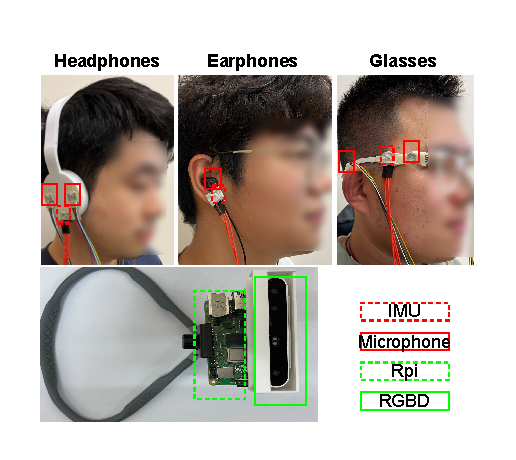
\includegraphics[width=1\linewidth]{chapters/egolog/figs/device.pdf}
    \vspace{-2em}
    \caption{Devices used in our data collection.}
    \vspace{-1em}
    \label{fig:egolog_device}
\end{figure}

\subsubsection{Public dataset}
To comprehensively evaluate EgoLog performance, we construct our dataset with the blow public datasets:

\paragraph{Ego4D:}
Ego4D \citep{grauman2022ego4d} is a large-scale dataset collected by various brands of head-mounted cameras (e.g., GoPro), offering synchronized multi-modal data (i.e., video, audio, and IMU signal). We consider the moment subset of the dataset, which consists of 158 classes. We can perform k-means clustering on the text embeddings to adapt to different levels of granularity. For the scenario annotation, we use the scenario annotation \citep{grauman2022ego4d} for each video since they have a similar definition. In total, there are 91 scenarios in the dataset. 
Considering Ego4D is the most diverse and large-scale dataset, we set it as the default dataset.

\paragraph{EgoADL:}
EgoADL \citep{sun2024multimodal} is also a large-scale dataset collected in the real world with Android smartphones, including Wi-Fi, audio, and IMU data. In this paper, we exclude Wi-Fi data for fair comparison. We perform a similar clustering for the 221 classes of actions in the dataset.

\paragraph{SAMOSA:}
SAMOSA \citep{mollyn2022samosa} is a relatively small-scale dataset collected by an Android smartwatch (i.e., Fossil Gen 5), including audio and IMU. There are 26 activities in total.

\subsubsection{Self-collected dataset}
The existing public datasets already include data from various devices—such as smart glasses, smartphones, and smartwatches—offering considerable duration and diversity. The purpose of our self-collected dataset is not to surpass these strengths but to address their limitations. Specifically, the spatial understanding discussed in Section \ref{sec:egolog_localization} relies on spatial audio, which is absent from the aforementioned datasets but is accessible using commercial devices. To compensate for this gap, we collected a new dataset featuring spatial audio recordings from different form factors: glasses, headphones, and earphones.

We constructed a dataset in which a volunteer acted as the user and a loudspeaker served as an audio interference source. The loudspeaker played audio samples from the NIGENS dataset \citep{trowitzsch2019nigens}, which contains 14 types of common sound events. The user, in contrast, performed the following 12 activities: standing up, sitting down, clapping, walking, talking, drinking, typing on a keyboard, eating, watching TV, washing hands, cleaning a room, and writing.
During data collection, the loudspeaker's position remained fixed. To simplify the experiment, the user's location was controlled for most activities (excluding walking), allowing us to manually record the relative position between the user and the loudspeaker. However, as users were not required to remain perfectly still, their precise position was not controlled with high accuracy. To ensure the dataset's validity, users were instructed to limit their positional variance to within the spatial resolution of our classification model. In essence, while the user's location was dynamic, the annotation was treated as static from the perspective of the classification task.
For the walking activity, where the relative position changes continuously, we used an RGB-D camera to perform Simultaneous Localization and Mapping (SLAM) to estimate the user's trajectory. This estimation was based on the assumption that the user started from a fixed, known position in the room (the location of the loudspeaker is also fixed and known).


\subsubsection{Baselines}
We adopt the following evaluation metrics in this paper. For the multi-label classification (i.e., scenario and spatial), we use the multi-label F1-Score: $2*TP/(2*TP+FP+FN)$. For the single-label classification (i.e., activity), we use the accuracy as the metric.

To evaluate our approach, EgoLog, we have selected different baselines for activity recognition and scenario recognition, respectively. Specifically, we consider SAMoSA \citep{mollyn2022samosa} and Imagebind \citep{girdhar2023imagebind} as our baselines for activity recognition, which are conventional supervised multi-modal model that accepts both audio and IMU. For the scenario recognition, both of the above baselines with larger data duration are considered. To ensure a fair comparison, all of them are fine-tuned with the same data.

\subsection{Activity Recognition}
\begin{figure}[h]
    \centering
    \begin{minipage}{0.48\linewidth}
        \centering
      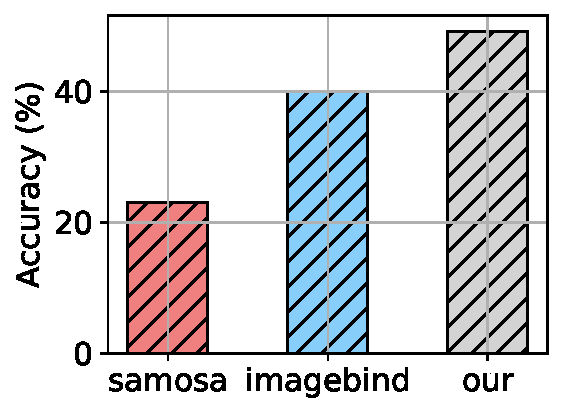
\includegraphics[width=1\linewidth]{chapters/egolog/eval/activity_ego4d.pdf}
          \vspace{-0.5em}
      \caption{Activity recognition on Ego4D.}
        \label{fig:egolog_activity_ego4d}
    \end{minipage}
    \hfill
    \begin{minipage}{0.48\linewidth}
        \centering
    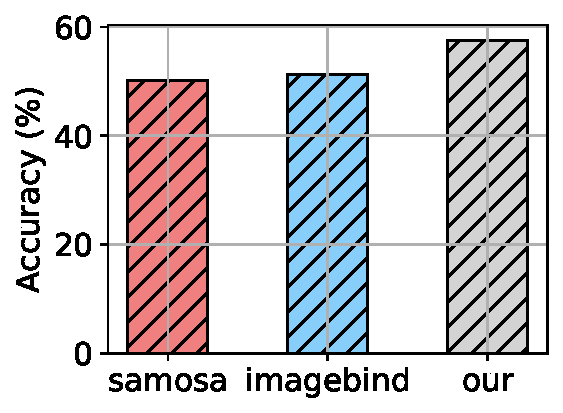
\includegraphics[width=1\linewidth]{chapters/egolog/eval/activity_egoadl.pdf}
        \vspace{-0.5em}
      \caption{Activity recognition on EgoADL.}
        \label{fig:egolog_activity_egoadl}
    \end{minipage}
    \vspace{-0.5em}
\end{figure}

\begin{figure}[h]
    \centering
    \begin{minipage}{0.48\linewidth}
        \centering
       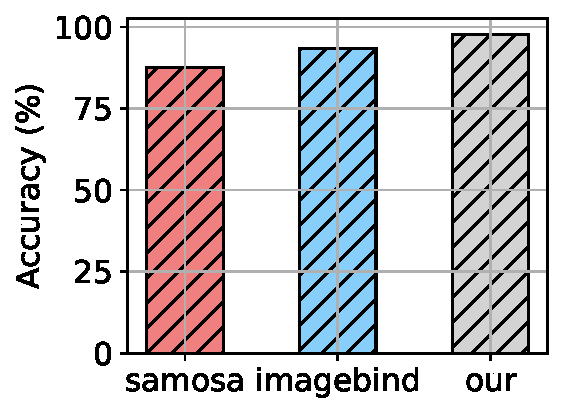
\includegraphics[width=1\linewidth]{chapters/egolog/eval/activity_samosa.pdf}
           \vspace{-0.5em}
      \caption{Activity recognition on SAMOSA.}
        \label{fig:egolog_activity_samosa}
    \end{minipage}
    \hfill
    \begin{minipage}{0.48\linewidth}
        \centering
    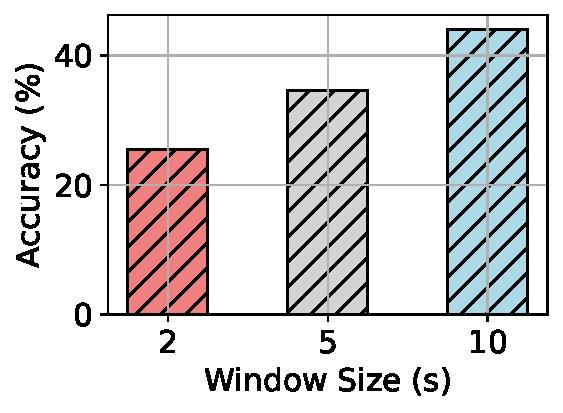
\includegraphics[width=1\linewidth]{chapters/egolog/eval/activity_window_size.pdf}
        \vspace{-0.5em}
      \caption{Activity recognition vs. data length.}
        \label{fig:egolog_activity_length}
    \end{minipage}
\vspace{-0.5em}
\end{figure}

We present the performance of our method for human activity recognition on the Ego4D, EgoADL, and SAMOSA datasets. As shown in Fig. \ref{fig:egolog_activity_ego4d}, \ref{fig:egolog_activity_egoadl}, and \ref{fig:egolog_activity_samosa}, our approach consistently outperforms the baselines, with the most notable improvement on the SAMOSA dataset.

The performance gap is most significant on the Ego4D dataset (23\% vs. 52\%), which is the most challenging. Compared to ImageBind, EgoLog achieves superior performance (52\% vs. 40\%) with significantly lower computational cost.

On the other two, less diverse datasets, the advantages of EgoLog are slightly reduced. We attribute this primarily to a lack of contextual information; Ego4D data was collected "in the wild," while the others were gathered in moderately controlled experimental settings. Despite this, our approach still outperforms the best baseline by 6\%on EgoADL and 4\%on SAMOSA, demonstrating its robustness. Note that the absolute accuracy for SAMOSA is the highest, which is expected as it has the smallest number of classes, making it the least challenging dataset.


\paragraph{Data length.}
Since the length of the data significantly influences both audio and IMU data, we first establish the hyperparameters before evaluating the system.
We present the performance of human activity recognition along with various data lengths, in Fig. \ref{fig:egolog_activity_length}. We observe that the HAR performance stays stable when the data length is larger than five seconds, while significantly dropping when the data length is one second. As a result, we keep the data length of HAR to five seconds. 

\begin{figure}[h]
    \centering
    \begin{minipage}{0.48\linewidth}
        \centering
       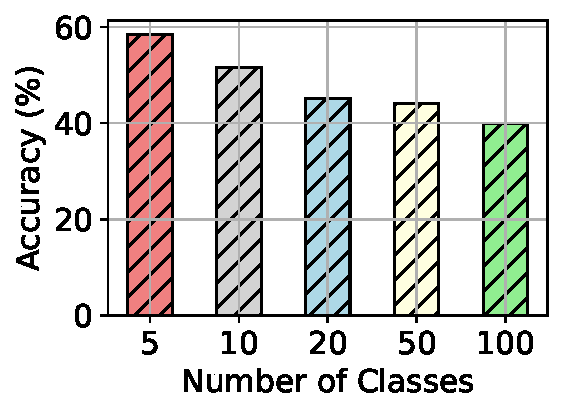
\includegraphics[width=1\linewidth]{chapters/egolog/eval/activity_num_classes.pdf}
           \vspace{-0.5em}
      \caption{Human activities recognition performance vs. number of classes.}
        \label{fig:egolog_activity_num_classes}
    \end{minipage}
    \hfill
    \begin{minipage}{0.48\linewidth}
        \centering
    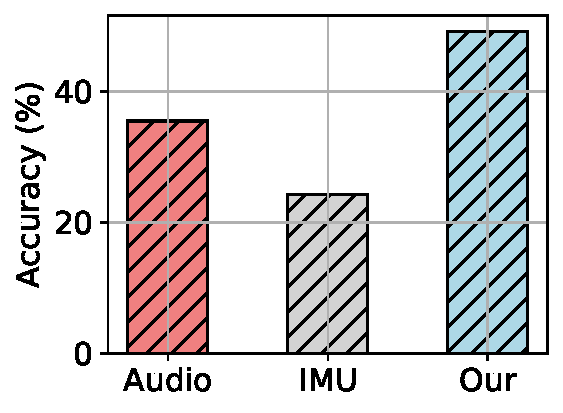
\includegraphics[width=1\linewidth]{chapters/egolog/eval/activity_modality.pdf}
        \vspace{-0.5em}
      \caption{Human activities recognition performance vs. modality.}
        \label{fig:egolog_activity_modality}
    \end{minipage}
\vspace{-0.5em}
\end{figure}

\paragraph{Number of classes.}
We split the sampled Ego4D dataset into activities and evaluated their performance in Fig. \ref{fig:egolog_activity_num_classes}. We observe that there are performance gaps between activities, indicating that the complexity of each of them is different. Specifically, we inspect the top three worst activities, which are putting something in a container or on a surface, cutting with scissors, and sleeping. We observe that they are both quiet, and the motion is weakly related to the head, so it is natural to have lower performance.

\paragraph{Modalities fusion.}
As shown in Figure \ref{fig:egolog_activity_modality}, our multi-modal fusion approach (audio+IMU) surpasses the audio-only and IMU-only baselines, improving activity recognition performance by more than 10\%.


\begin{table}[h]
\centering
\caption{Ablation study on activity recognition for different datasets, the metric is accuracy.}
\label{tab:ab_activity}
\begin{tabular}{ccccc}
\toprule
\textbf{Model}  & \textbf{Ego4D$\uparrow$} & \textbf{EgoADL$\uparrow$} & \textbf{SAMOSA$\uparrow$} \\
\midrule
Random  & 0.02 & 0.02 & 0.04 \\
\midrule
ImageBind-FT  & 0.40 & 0.51 & 0.93 \\
\midrule
Multi-modal & 0.401 & 0.49 & 0.90\\
+ Scenario & \textbf{0.467} & \textbf{0.58} & \textbf{0.97} \\
\bottomrule
\end{tabular}
\end{table}

\paragraph{Ablation study.}
We conduct an ablation study on different components of our system, including each modality (audio and IMU), multi-modal fusion, scenario as condition, and scenario as condition via Imagebind-embedding, as shown in Tab. \ref{tab:ab_activity}. For reference, we also list the performance of a random guess (indicating the number of classes) and baseline ImageBind-FT.
We observe that


\subsection{Scenario Recognition}
\begin{figure}[h]
    \centering
    \begin{minipage}{0.48\linewidth}
        \centering
    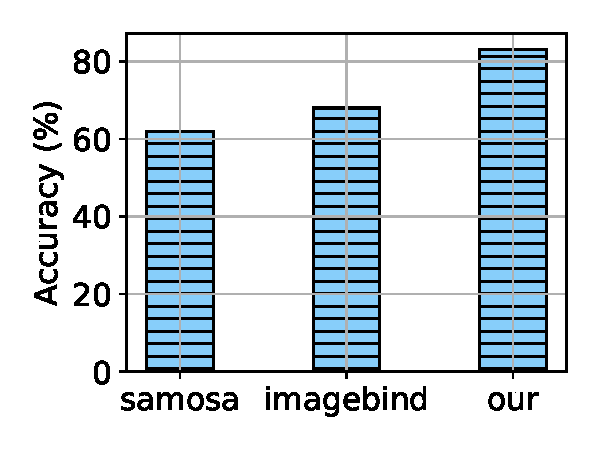
\includegraphics[width=1\linewidth]{chapters/egolog/eval/scenario_cls.pdf}
           \vspace{-0.5em}
      \caption{Scenario recognition accuracy on Ego4D.}
        \label{fig:egolog_scenario}
    \end{minipage}
    \hfill
    \begin{minipage}{0.48\linewidth}
        \centering
    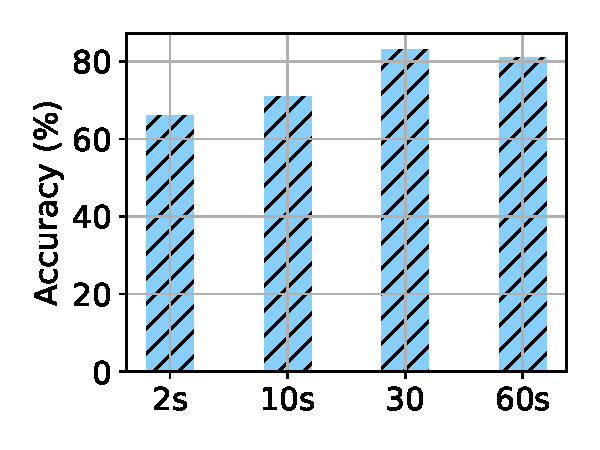
\includegraphics[width=1\linewidth]{chapters/egolog/eval/scenario_length.pdf}
        \vspace{-0.5em}
      \caption{Scenario recognition accuracy vs. data length.}
        \label{fig:egolog_scenario_length}
    \end{minipage}
    \vspace{-0.5em}
\end{figure}



\begin{figure}[h]
    \centering
    \begin{minipage}{0.48\linewidth}
        \centering
      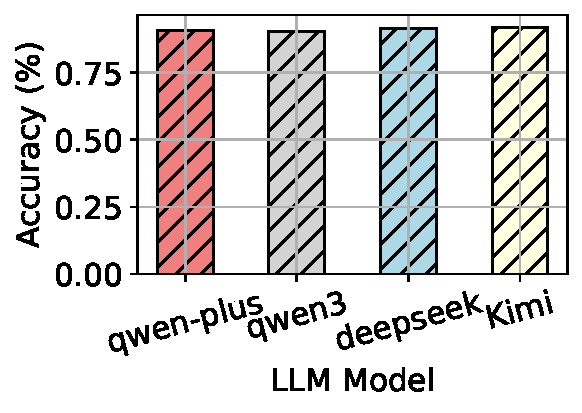
\includegraphics[width=\linewidth]{chapters/egolog/eval/scenario_llm_model.pdf}
          \vspace{-0.5em}
     \caption{Selection of LLM.}
    \label{fig:egolog_selection_llm}
    \end{minipage}
    \hfill
    \begin{minipage}{0.48\linewidth}
     \begin{tabular}{cc}
        \toprule
        \textbf{Model} & \textbf{Ego4D$\uparrow$} \\
        \midrule
        Random & 0.01\\
        \midrule
        Multi-modal & 0.70 \\
        + Contrastive & 0.83\\
        + Transformer  & 0.85 \\
        + LLM feedback  & 0.90\\
        \bottomrule
        \end{tabular}
        \vspace{1em}
        \captionof{table}{Ablation study on scenario recognition.}
        \label{tab:ab_scenario}
    \end{minipage}
    \vspace{-0.5em}
\end{figure}


Recalled in Sec. \ref{sec:egolog_scenario}, we employ a two-stage model to recognize the scenario by extracting the key-frame. In comparison, we consider audio scene recognition and ImageBind-IMU, which are audio-only and IMU-only methods
as the two baselines shown in Fig. \ref{fig:egolog_scenario}. We observe that our method outperforms the two baselines by 15\%, indicating that our long-time multi-modal fusion works well for scenario recognition. 

\paragraph{Data length.}
Based on our earlier definitions, scenarios that require capturing long-term information should use longer data lengths. We present the performance of scenario recognition along with various data lengths in Fig. \ref{fig:egolog_scenario_length}. We observe that the ideal data length is set to 30 seconds since the larger input data can reduce the performance.

\paragraph{Selection of LLM.}
Since our design is compatible with any LLM, we evaluated the performance using different LLMs from various sources. As shown in Fig. \ref{fig:egolog_selection_llm}, we observe that the performance is similar across them, indicating that common LLMs are sufficient for our design. For better deployment, we plan to explore the use of smaller LLMs in the future to reduce costs.

\paragraph{Ablation study.}
We conducted an ablation study to evaluate the contribution of different components in our system, including contrastive learning, the transformer module, and the addition of LLM feedback. The results are presented in Tab. \ref{tab:ab_scenario}. For reference, we also include the performance of a random guess (based on the number of classes).

Our observations indicate that contrastive learning is the most effective component, providing the largest performance improvement (13\%). The LLM feedback, facilitated by edge-cloud collaboration, yields a further, albeit smaller, gain. Given that LLM feedback is less susceptible to cross-domain variations, we consider this slight improvement to be meaningful.



\subsection{Spatial Understanding for Scenario Recognition}
\begin{figure}[h]
    \centering
    \begin{minipage}{0.48\linewidth}
         \centering
    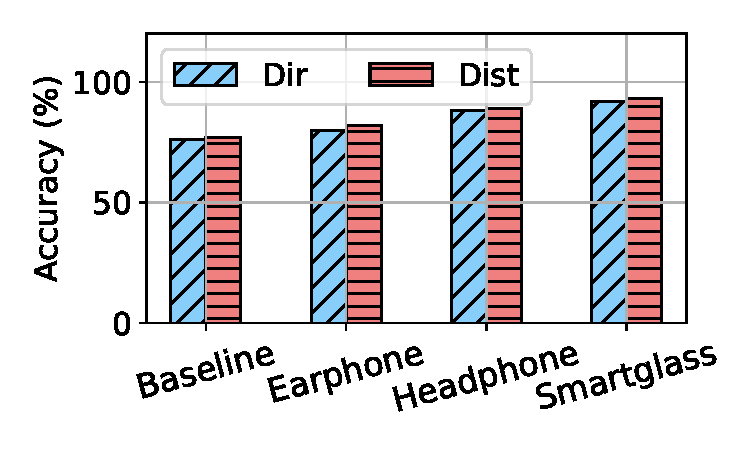
\includegraphics[width=1\linewidth]{chapters/egolog/eval/sound_localization.pdf}
            \vspace{-0.5em}
      \caption{Sound localization accuracy.}
        \label{fig:egolog_sound_localization}
    \end{minipage}
    \hfill
    \begin{minipage}{0.48\linewidth}
        \centering
    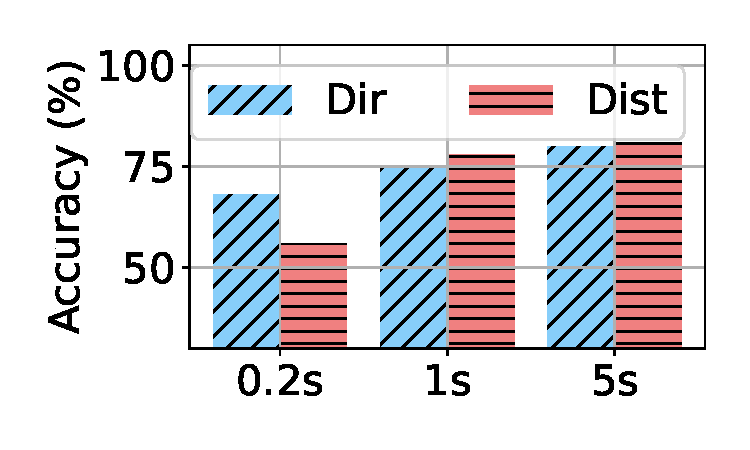
\includegraphics[width=1\linewidth]{chapters/egolog/eval/sound_localization_length.pdf}
          \vspace{-0.5em}
    \caption{Sound localization accuracy vs. data length.}
    \label{fig:egolog_sound_localization_length}
    \end{minipage}
    \vspace{-0.5em}
\end{figure}

\begin{figure}[h]
  \centering
  \begin{minipage}{0.4\linewidth}
    \centering
    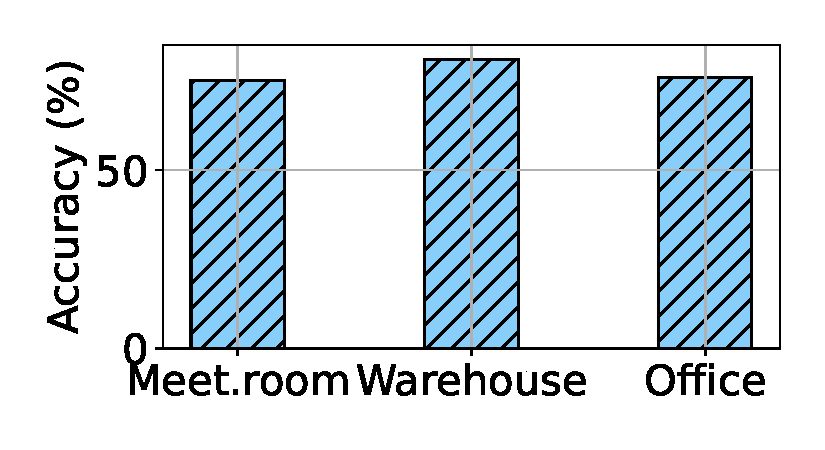
\includegraphics[width=1\linewidth]{chapters/egolog/eval/sound_localization_place.pdf}
        \vspace{-0.5em}
      \caption{Sound localization accuracy at different places.}
        \label{fig:egolog_sound_localization_place}
  \end{minipage}
  \hfill
  \begin{minipage}{0.58\linewidth}
    \centering
     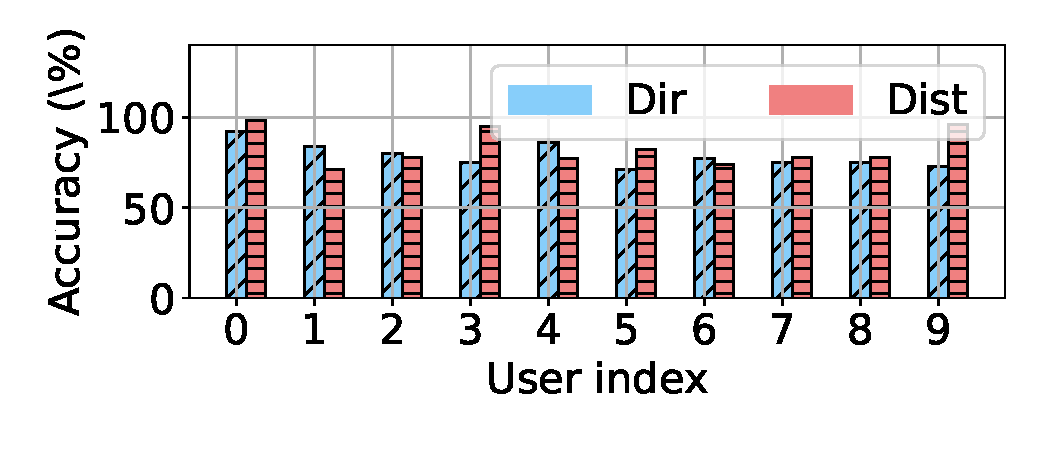
\includegraphics[width=1\linewidth]{chapters/egolog/eval/sound_localization_user.pdf}
         \vspace{-0.5em}
      \caption{Binaural sound localization accuracy for different users.}
        \label{fig:egolog_sound_localization_user}
  \end{minipage}
\vspace{-0.5em}
\end{figure}
In Fig. \ref{fig:egolog_sound_localization}, we compare the baseline (without motion compensation) with our proposed method across different devices. We report the accuracy for both direction (Dir) and distance (Dist) separately. The results show that our method improves accuracy by approximately 10\%when using IMU data for motion compensation.

Regarding performance across devices, we observe a consistent improvement from binaural earphones to 4-channel headphones and further to 4-channel smart glasses, which aligns with our expectations. In the following section, we will focus on evaluating data from earphones, which exhibit the lowest performance.

\paragraph{Data length.}
Since the length of the audio significantly influences the performance of sound localization, we test the accuracy with different length of data in Fig. \ref{fig:egolog_sound_localization_length}. According to the result, we set the data length of sound localization to one second to balance the latency and accuracy.

\paragraph{Different environments.}
We conducted further assessments of localization accuracy across various environments, such as distinct rooms. Room layout and object configurations induce varying room impulse responses, affecting recordings in conjunction with HRTFs. Our performance evaluation across different rooms is presented in Figure \ref{fig:egolog_sound_localization_place}, demonstrating that our model maintains consistent performance across diverse settings.

\paragraph{Different users.}
Binaural sound localization depends on individual-specific HRTFs, rendering neural networks calibrated for one user
ineffective for others. We assess personalized models across a group of users and present the overall accuracy in Figure 21. Despite performance variations among users, consistent accuracy (>75\%) is maintained within the group

\subsection{User Study}

% \begin{table}[h]
% \centering
% \vspace{-0.5em}
% \caption{User study.}
% \label{tab:user_study}
% \begin{tabular}{ll}
% \toprule
% \textbf{Question} & \textbf{EgoLog}\\
% \midrule
% Correctness &  \\
% Information-richness & \\
% User-friendly & \\
% \bottomrule
% \end{tabular}
% \vspace{-0.5em}
% \end{table}

To evaluate the benefits of EgoLog from a user perspective, we conducted a study where volunteers provided subjective ratings of the system's outputs. Recall that our goal is to provide users with a daily log that comprehensively summarizes and represents their activities through two complementary types of output: scenarios and activities. 
Our final solution integrates both outputs: the daily log displays two rows, with the first row showing scenario information and the second row presenting activity data. Since scenarios are recognized every 30 seconds, the output can contain errors or inconsistencies, even within the same scenario. To mitigate this, we represent each scenario using the normalized probability calculated from the most recent 10 minutes of data. 
For activities, due to the larger volume of data, we present the results using a bar chart with activity names labeled at the bottom.
Users were asked to rate the outputs based on three criteria: Correctness, Information-richness, and User-friendliness. To assess correctness, they were provided with ground-truth data in the same format. The average ratings (on a scale of 1-min to 5-max) for the three dimensions were 4.5, 4.0, and 4.5, respectively.


\subsection{Overhead}
While our system is not specifically designed for real-time responses, it is crucial to maintain low resource consumption.

\begin{table}[h]
\centering
\vspace{-0.5em}
\caption{Model runtime latency.}
\vspace{-0.5em}
\label{tab:latency}
\begin{tabular}{llcc}
\toprule
\textbf{Section} & \textbf{Interval} & \textbf{CPU} & \textbf{GPU} \\
\midrule
Scenario & 30 seconds & 0.55s & 9ms \\
Spatial & 2 seconds & 2.5ms & 2.1ms \\
HAR  & 10 seconds & 34ms & 2.7ms \\
\bottomrule
\end{tabular}
\vspace{-0.5em}
\end{table}

\paragraph{Latency.}
EgoLog comprises three core components: (1) scenario recognition (Sec. \ref{sec:egolog_scenario}), (2) sound localization (Sec. \ref{sec:egolog_localization}), and (3) HAR (Sec. \ref{sec:egolog_har}). As shown in Tab. \ref{tab:latency}, most components are lightweight, enabling real-time performance on both CPU and GPU platforms. Notably, scenario recognition on CPU requires 0.55 seconds but is executed once every 30 seconds, rendering its latency negligible. While EgoLog does not mandate real-time user feedback, lower latency enhances user experience by minimizing wait times.


\paragraph{Power consumption.}
To evaluate our power consumption, we locked the screen while continuously recording both audio and IMU data. We then checked the battery level before and after one hour of recording. Using the Pixel 7 as a reference, we observed approximately a 5\% drop in power after one hour of recording. Given that there is potential for further optimization, EgoLog shows promise for effective long-term operation.

\paragraph{Data storage.}
We record audio at a sample rate of 48 kHz, with a 16-bit depth and 2 channels, resulting in a compressed file size of about 170-210 kbps in MP3 format. This equates to around 70 MB of audio data per hour. For motion data, with an update rate set to 10 Hz, the size in CSV format is approximately 1 kB per second, leading to around 3 MB of data per hour.
As a result, we can process this data periodically, ensuring that storage requirements remain manageable and do not become overwhelming.





The system's privacy boundary and deployment safeguards are discussed in Section~\ref{sec:thesis_privacy}.
